%!TEX TS-program = xelatex
\documentclass{beamer}

\usepackage{HSE-theme/beamerthemeHSE} % Подгружаем тему

%%% Работа с русским языком и шрифтами
\usepackage{xecyr}   % загружает пакет многоязыковой вёрстки
\usepackage{cancel}
\usepackage{amsmath}
\usepackage{fontspec}      % подготавливает загрузку шрифтов Open Type, True Type и др.
\defaultfontfeatures{Ligatures={TeX},Renderer=Basic}  % свойства шрифтов по умолчанию
\setmainfont[Ligatures={TeX,Historic}]{Arial} %  установите шрифты Myriad Pro или (при невозможности) замените здесь на другой шрифт, который есть в системе — например, Arial
\setsansfont{Arial}  %  установите шрифты Myriad Pro или (при невозможности) замените здесь на другой шрифт, который есть в системе — например, Arial
\setmonofont{Courier New}
\uselanguage{russian}
\languagepath{russian}
\deftranslation[to=russian]{Theorem}{Теорема}
\deftranslation[to=russian]{Definition}{Определение}
\deftranslation[to=russian]{Definitions}{Определения}
\deftranslation[to=russian]{Corollary}{Следствие}
\deftranslation[to=russian]{Fact}{Факт}
\deftranslation[to=russian]{Example}{Пример}
\deftranslation[to=russian]{Examples}{Примеры}

\usepackage{multicol} 		% Несколько колонок
\graphicspath{{images/}}  	% Папка с картинками
\usepackage{tikz}

% Мое
\newcommand{\relu}{\operatorname{relu}}
\newcommand{\softmax}{\operatorname{softmax}}
\newcommand{\sigmoid}{\operatorname{sigmoid}}
\usepackage{caption}
\usepackage{mathtools}
\usepackage{tikz}
\makeatletter
\newcommand\mathcircled[1]{%
  \mathpalette\@mathcircled{#1}%
}

\newcommand\@mathcircled[2]{%
  \tikz[baseline=(math.base)] \node[draw,circle,inner sep=1pt] (math) {$\m@th#1#2$};%
}
\makeatother

\usepackage{mathrsfs}



\tikzstyle{format} = [thick,
                      minimum size=1cm,
                      draw=blue!50!black!50,
                      top color=white,
                      bottom color=blue!50!black!20,
                      ]

\newcommand{\R} {\mathbb{R}}
\newcommand{\Sum}[2]{\overset{#2}{\underset{#1}{\sum}}}



%%% Информация об авторе и выступлении
\title[Нейронные сети с нуля]{Нейронные сети с нуля}
\subtitle{Программный проект \\ Факультет компьютерных наук}
\author[Гимранов Артур БПМИ204]{Гимранов Артур, БПМИ204 \\ \scriptsize{Научный руководитель: к.ф.-м.н., доцент Трушин Дмитрий Витальевич}}
\institute[Высшая школа экономики]{Национальный исследовательский университет \\ «Высшая школа экономики» (Москва)}
\date{Июнь 2022}

\begin{document}	% Начало презентации

\frame[plain]{
    \titlepage
}	% Титульный слайд

\begin{frame}{Постановка задачи}
\large{
    \begin{itemize}
        \large{
            \item Изучить теорию нейросетей и градиентного спуска \pause
            \item Имплементировать необходимые классы и структуры \pause
            \item Протестировать на реальных данных
        }
    \end{itemize}
}
\end{frame}

\begin{frame}{Структура нейронной сети}
    \begin{figure}[h]
        \center{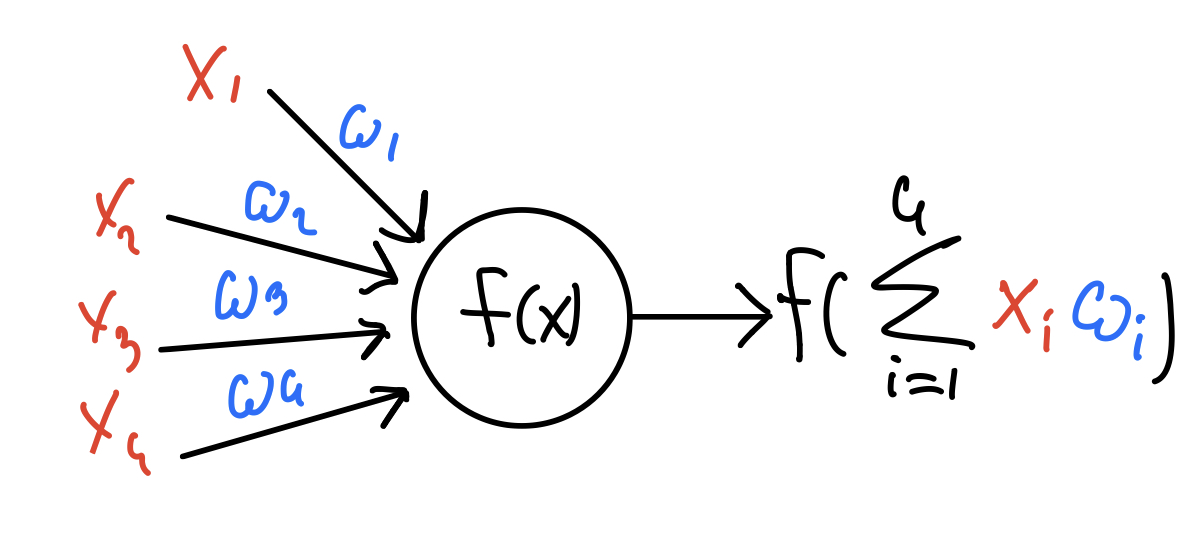
\includegraphics[scale=0.1]{../TermPaper/pictures/neuron.jpeg}}
    \end{figure} \pause
    \begin{figure}[h]
        \center{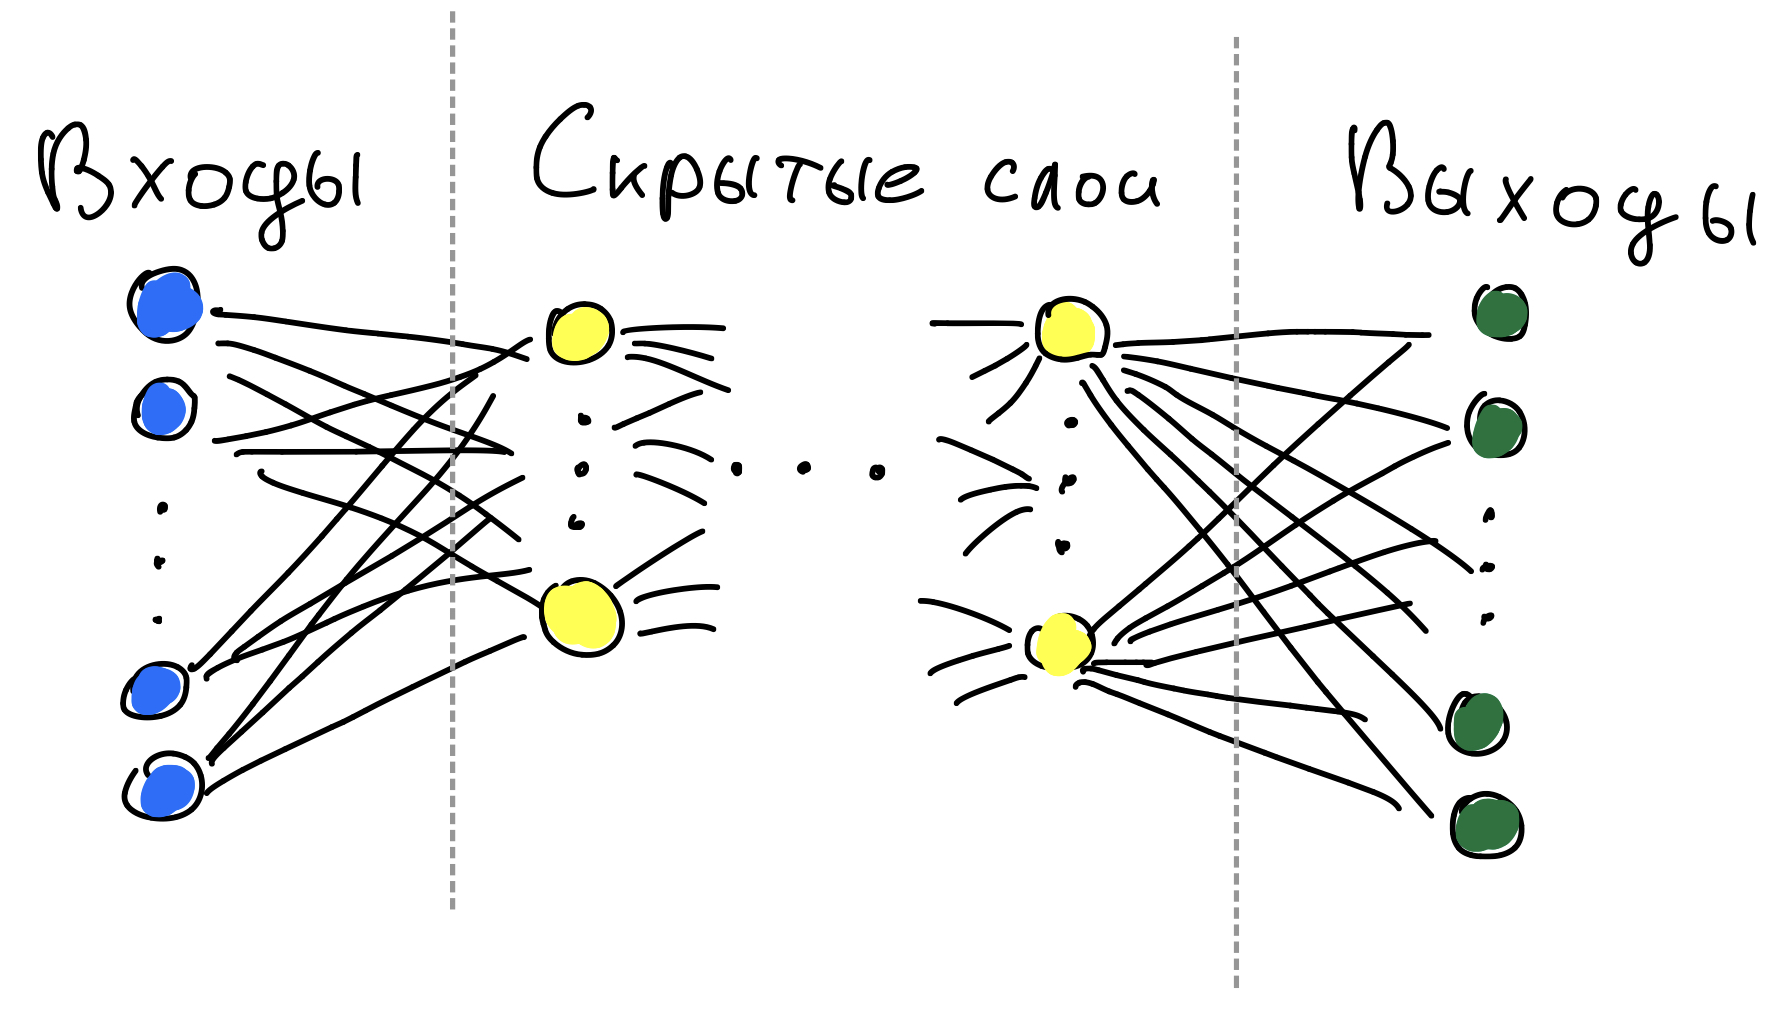
\includegraphics[scale=0.14]{../TermPaper/pictures/structure.jpeg}}
    \end{figure}
\end{frame}

\begin{frame}{Интерпретация}
        \begin{enumerate}
            \item Веса связей лежат в матрице A \pause
            \item Смещение лежит в векторе b \pause
            \item f -- функция активации \pause
            \begin{enumerate}
                \item $\softmax$
                \item $\relu$
                \item $\sigmoid$
            \end{enumerate} \pause
            \item Весь выход слоя $f(Ax + b)$ \pause
        \end{enumerate}
        \begin{center}
            Зададим слой блоком, который хранит $\theta = (A, b)$ и $f$. $g(x, \theta) = f(Ax + b)$

            $$
                \R^n \xrightarrow[]{x} \underset{g(x, \theta)}{\boxed{\theta}} \xrightarrow[]{y} \R^m
            $$
        \end{center}
\end{frame}

\begin{frame}{Задача}
    \begin{itemize}
        \item В $x$ лежат $k$ признаков, $x = [x^{(1)}, \dots, x^{(k)}]^t$ \pause
        \item В $y$ лежат $l$ признаков, $y = [y^{(1)}, \dots, y^{(l)}]^t$ \pause
        \item Начальная выборка $\forall i \le n: x_i \rightarrow y_i$ \pause
    \end{itemize}

    \begin{center}
        Хотим найти $F(x) = y$. Будем искать $F$ в виде нейросети. \pause
        $$
        \R^k \xrightarrow[]{x_i} \underset{g_1(x, \theta_1)}{\boxed{\theta_1}} \xrightarrow[]{w_i} \underset{g_2(x, \theta_2)}{\boxed{\theta_2}} \xrightarrow[]{z_i} \R^l
        $$
        Функция ошибки
        $$
        \phi(\theta_1, \theta_2) = \frac{1}{n}\Sum{i = 1}{n} \|g_2(g_1(x_i, \theta_1), \theta_2) - y_i\|^2 \rightarrow \underline{\min}_{\theta_1, \theta_2}
        $$
        Минимум по $\theta_1, \theta_2$ найдем градиентным спуском
        \end{center}
\end{frame}

\begin{frame}{Обучение}
    \center{Функция ошибки для всей сети}
    $$
    \phi(\Theta) = \frac{1}{n} \Sum{i = 1}{n} \mathscr{L}(z_i, y_i)
    $$
    \center{Прямым обходом мы считаем все выходы и ошибку}
    $$
    \underleftarrow{
    \overrightarrow{
    \R^n \rightarrow \underset{g_1(x, \theta_1)}{\boxed
    {\theta_1}} \rightarrow \dots \rightarrow \underset{g_i(x, \theta_i)}{\boxed{\theta_i}} \rightarrow \dots \rightarrow \underset{g_k(x, \theta_k)}{\boxed
    {\theta_k}} \overset{z_i}{\rightarrow} \mathcircled{\mathscr{L}} \rightarrow \R
    }
    }
    $$
    \center{Обратным проходом считаем градиенты $\frac{\partial \phi}{\partial \theta_i}$}
\end{frame}

% \begin{frame}{Алгоритм обучения}
%     Что хотим:
%     \begin{enumerate}
%         \item Навесить функцию потерь
%         \item Посчитать градиент от функции потерь по всем параметрам
%         \item Сдвинуть параметры против градиента
%         \item Таким образом уменьшать ошибку на обучающей выборке
%     \end{enumerate}
%     \begin{enumerate}
%         \item Пройтись вперед посчитать предсказание и ошибку
%         \item Посчитать градиент
%     \end{enumerate}
% \end{frame}

\begin{frame}{Архитектура}
    \begin{enumerate}
        \item \texttt{Net}. Инцилизирует ресурсы, обучает и предсказывает. \pause
        \item \texttt{ComputeBlock}. Наши слои (блоки). Содержит функцию активации и параметры. Вычисляет функцию и необходимые градиенты. \pause
        \item \texttt{LossFunction}. Функция ошибок, нужна для расчета отклонения и вычисления градиента \pause
        \item \texttt{ActivationFunction}. Класс родитель для функций активации, имеет виртуальные методы для вычисления функции и ее производной в точке.
            \begin{enumerate}
                \item \texttt{Sigmoid}
                \item \texttt{Relu}
                \item \texttt{Softmax}
            \end{enumerate}
    \end{enumerate}
\end{frame}

\begin{frame}{Тесты}
    \begin{center}
        Нейросеть тестировалась на популярном датасете mnist.
        Точность составила более 90\% при 12 минутах обучения на CPU
    \end{center}
\end{frame}


\begin{frame}{Тесты}
    \center{Условия тестирования:}
    \begin{itemize}
        \item Выборка из 8500 изображений рукописных цифр \pause
        \item Входной слой состоял из 784 нейронов, каждый из которых отвечал за пиксель в картинке $28 \times 28$, с функцией активации $\relu$ \pause
        \item Первый скрытый слой состоял из 16 нейронов, с функцией активации $\relu$ \pause
        \item Второй скрытый слой состоял из 16 нейронов, с функцией активации $\softmax$ \pause
        \item Выходной слой состоял из 10 нейронов \pause
        \item Количество эпох (итераций обучения) = 3000 \pause
        \item Learning rate (шаг градиентного спуска) = 0.6 \pause
        \item Размер батча 128 \pause
        \item Функция потерь MSE
    \end{itemize}
\end{frame}

\begin{frame}{The end}
    \centering
        Спасибо за внимание!
        \begin{figure}[t]
        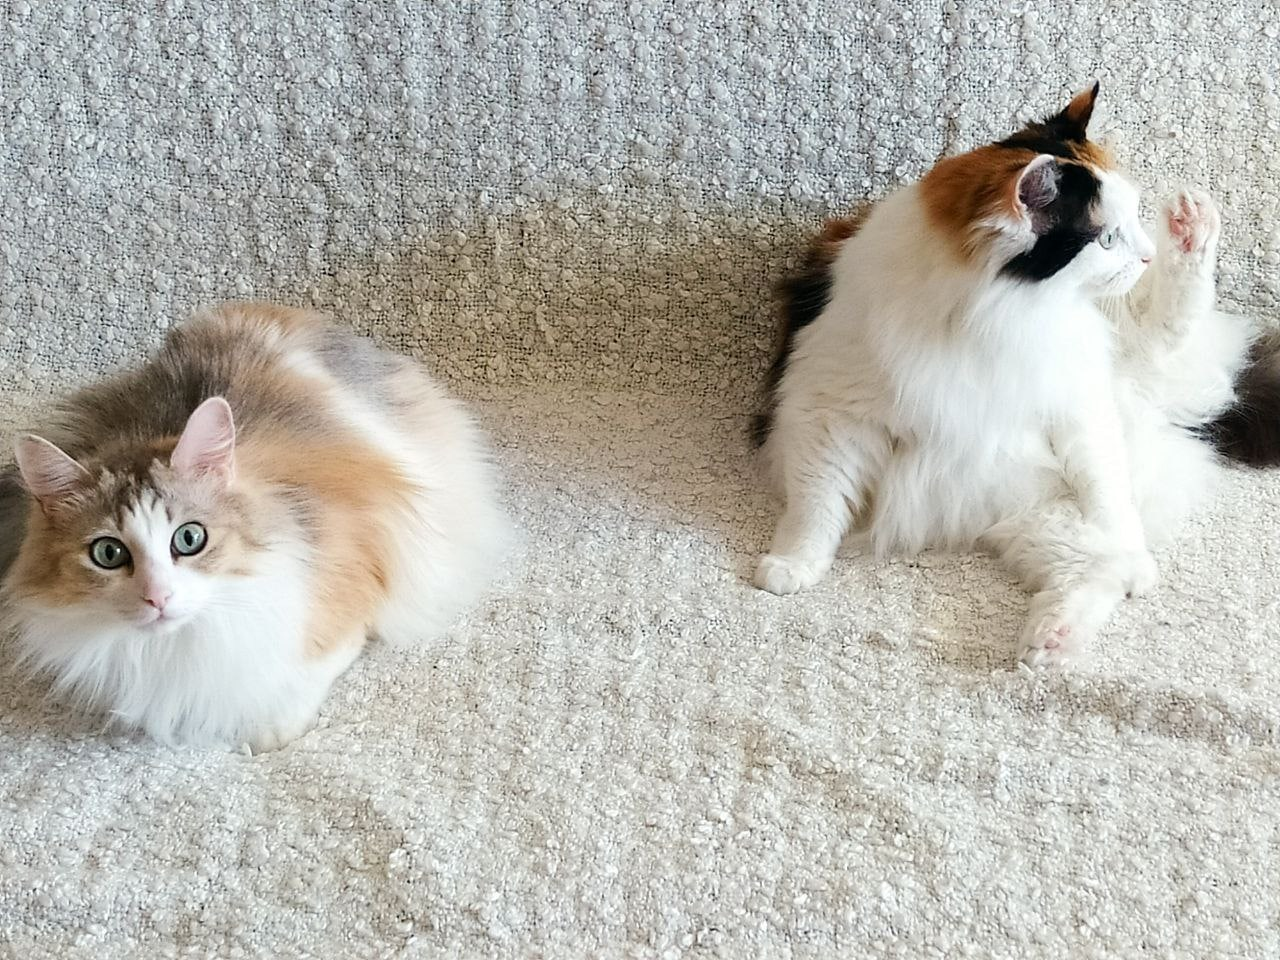
\includegraphics[scale=0.17]{cats.jpg}
            \centering
        \end{figure}
    \end{frame}

% \begin{frame}{Идея IF4}
%     Алгоритм F4:
%     \begin{enumerate}
%         \item Для $\cancelto{\text{всех множеств пар}}{\text{каждой пары}}$ многочленов составить их $S$-полиномы и найти их остаток по этому множеству.
%         \item Если все остатки равны нулю и все пары рассмотрены, получен базис Грёбнера. Иначе, добавить все ненулевые остатки во множество и вернуться к шагу 1.
%     \end{enumerate}
% \end{frame}

% \begin{frame}{Идея IF4}
%     Алгоритм IF4:
%     \begin{enumerate}
%         \item Для $\cancelto{\cancelto{\text{некоторого множества пар}}{\text{всех множеств пар}}}{\text{каждой пары}}$ многочленов составить их $S$-полиномы и найти их остаток по этому множеству.
%         \item Если все остатки равны нулю и все пары рассмотрены, получен базис Грёбнера. Иначе, добавить некоторые ненулевые остатки во множество и вернуться к шагу 1.
%     \end{enumerate}
% \end{frame}

% \begin{frame}{Идея IF4}
%     Алгоритм IF4:
%     \begin{enumerate}
%         \item Для $\cancelto{\cancelto{\text{\underline{некоторого} множества пар}}{\text{всех множеств пар}}}{\text{каждой пары}}$ многочленов составить их $S$-полиномы и найти их остаток по этому множеству.
%         \item Если все остатки равны нулю и все пары рассмотрены, получен базис Грёбнера. Иначе, добавить \underline{некоторые} ненулевые остатки во множество и вернуться к шагу 1.
%     \end{enumerate}
% \end{frame}

% \begin{frame}{Идея IF4}
%     Алгоритм IF4:
%     \begin{enumerate}
%         \item Для $\cancelto{\cancelto{\text{\underline{некоторого} множества пар}}{\text{всех множеств пар}}}{\text{каждой пары}}$ многочленов составить их $S$-полиномы и \underline{\text{найти их остаток по этому множеству}}.
%         \item Если все остатки равны нулю и все пары рассмотрены, получен базис Грёбнера. Иначе, добавить \underline{некоторые} ненулевые остатки во множество и вернуться к шагу 1.
%     \end{enumerate}
% \end{frame}

% \begin{frame}{Редукция в IF4}
%     \begin{enumerate}
%         \item Подготовить всевозможные редукторы. Возможно, как-то предварительно упростить их. \pause
%         \item Матрички -- наше всё! \pause
%     \end{enumerate}
%     $$
%     \begin{matrix}
%         \  & \begin{matrix}\ m_1&m_2&m_3&\ldots&m_n\end{matrix} \\
%         \begin{matrix}
%             f_1 \\ f_2  \\ f_3 \\ \ldots \\ f_{k-1} \\ f_{k}
%         \end{matrix} &
%         \begin{pmatrix}
%             \times & \times & \times & \ldots & \times \\
%             \times & \times & \times & \ldots & \times \\
%     		\times & \times & \times & \ldots & \times \\
%             \ldots & \ldots & \ldots & \ldots & \ldots \\
%             \times & \times & \times & \ldots & \times \\
%             \times & \times & \times & \ldots & \times \\
%         \end{pmatrix}
%     \end{matrix} \pause \longrightarrow
%     \begin{pmatrix}
%         1 & 0 & ... & 0 & \times & ... & \times \\
%         0 & 1 & ... & 0 & \times & ... & \times \\
%         ... & ... & ... & ... & ... & ... & ... \\
% 		0 & 0 & ... & 1 & \times & ... & \times \\
%         0 & 0 & ... & 0 & 0 & ... & 0 \\
%         ... & ... & ... & ... & ... & ... & ... \\
%         0 & 0 & ... & 0 & 0 & ... & 0 \\
%     \end{pmatrix}
%     $$ \pause
%     И никаких бинарных операций с многочленами!
% \end{frame}

% \begin{frame}{Примерчик}
%     Рассмотрим Root3 над $\mathbb{R}[x, y, z]$ с лекс. порядком: $F = \{f_1 = x + y + z, f_2 = xy + xz + yz, f_3 = xyz - 1\}.$  \pause
%     \begin{enumerate}
%         \item После предобработки: $F = \{f_1\}, P = \{p_{1, 2}, p_{2, 3}\}$. \pause
%         \item Множество выбранных пар: $\{p_{1, 2}\}$. \pause
%         \item Всевозможные редукторы и редуцируемые многочлены: $\{yf_1, f_2, zf_1\}$. \pause
%         \item Множество мономов: $\{xy, xz, y^2, yz, z^2\}$ и матричка:
%         $$
%             \begin{pmatrix}
%                 1&1&0&1&0 \\
%                 1&0&1&1&0 \\
%                 0&1&0&1&1
%             \end{pmatrix}
%             \to
%             \begin{pmatrix}
%                 1&0&0&0&-1 \\
%                 0&1&0&1&1 \\
%                 0&0&1&1&1
%             \end{pmatrix}.
%         $$ \pause
%     \item Отредуцированное множество: $\{f_4 = xy - z^2, f_5 = xz + yz +z^2, f_6 = y^2 + yz + z^2\}$ и множество остатков: $\{f_6\}$.
%     \end{enumerate}

% \end{frame}


% \begin{frame}{Примерчик}
%     \begin{enumerate}
%         \setcounter{enumi}{5}
%         \item После обработки: $F = \{f_1, f_6\}, P = \{p_{2, 3}\}$. \pause
%         \item Множество выбранных пар: $\{p_{2, 3}\}$. \pause
%         \item Всевозможные редукторы и редуцируемые многочлены: $\{zf_2, zf_4\}$. \pause
%         \item Множество мономов: $\{xyz, z^3, 1\}$ и матричка:
%         $$
%             \begin{pmatrix}
%                 1&-1&0\\
%                 1&0&-1
%             \end{pmatrix}
%             \to
%             \begin{pmatrix}
%                 1&0&-1\\
%                 0&1&-1
%             \end{pmatrix}.
%         $$ \pause
%     \item Отредуцированное множество: $\{f_7 = xyz - 1, f_8 = z^3 - 1\}$ и множество остатков: $\{f_8\}$.\pause
%     \item После обработки: $F = \{f_1, f_6, f_8\}, P = \varnothing$.\pause
%     \end{enumerate}
%     Итоговый базис Грёбнера: $\{x + y + z, y^2 + yz + z^2, z^3 - 1\}$.

% \end{frame}



% \begin{frame}{Реализация}
%     Репозиторий: \href{https://github.com/cdraugr/GroebnerBasis}{https://github.com/cdraugr/GroebnerBasis}. \\
% \vspace{0.7cm}
%     Многочлены и множество многочленов:
%     \begin{figure}[t]
%         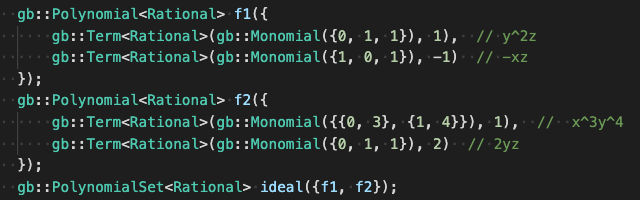
\includegraphics[scale=0.5]{PolSet.png}
%         \centering
%     \end{figure}
% \end{frame}

% \begin{frame}{Реализация}
%     Репозиторий: \href{https://github.com/cdraugr/GroebnerBasis}{https://github.com/cdraugr/GroebnerBasis}. \\
% \vspace{0.7cm}
%     Как считать базис Грёбнера, используя IF4:
%     \begin{figure}[t]
%         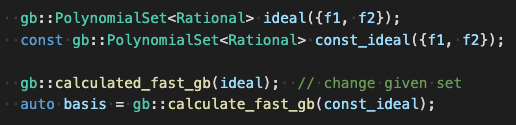
\includegraphics[scale=0.6]{HowToUse.png}
%         \centering
%     \end{figure}
% \end{frame}

% \begin{frame}{Реализация}
%     Репозиторий: \href{https://github.com/cdraugr/GroebnerBasis}{https://github.com/cdraugr/GroebnerBasis}. \\
% \vspace{0.7cm}
%     Как считать базис Грёбнера, используя IF4 и свою селекторную стратегию:
%     \begin{figure}[t]
%         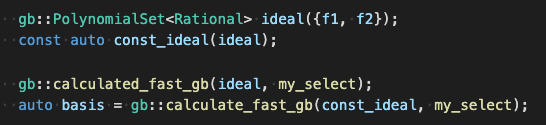
\includegraphics[height=3cm, width=11cm]{HowToUse2.png}
%         \centering
%     \end{figure}
% \end{frame}

% \begin{frame}{Пример вывода}
%     Базис Грёбнера для Root4:
%     \begin{figure}[t]
%         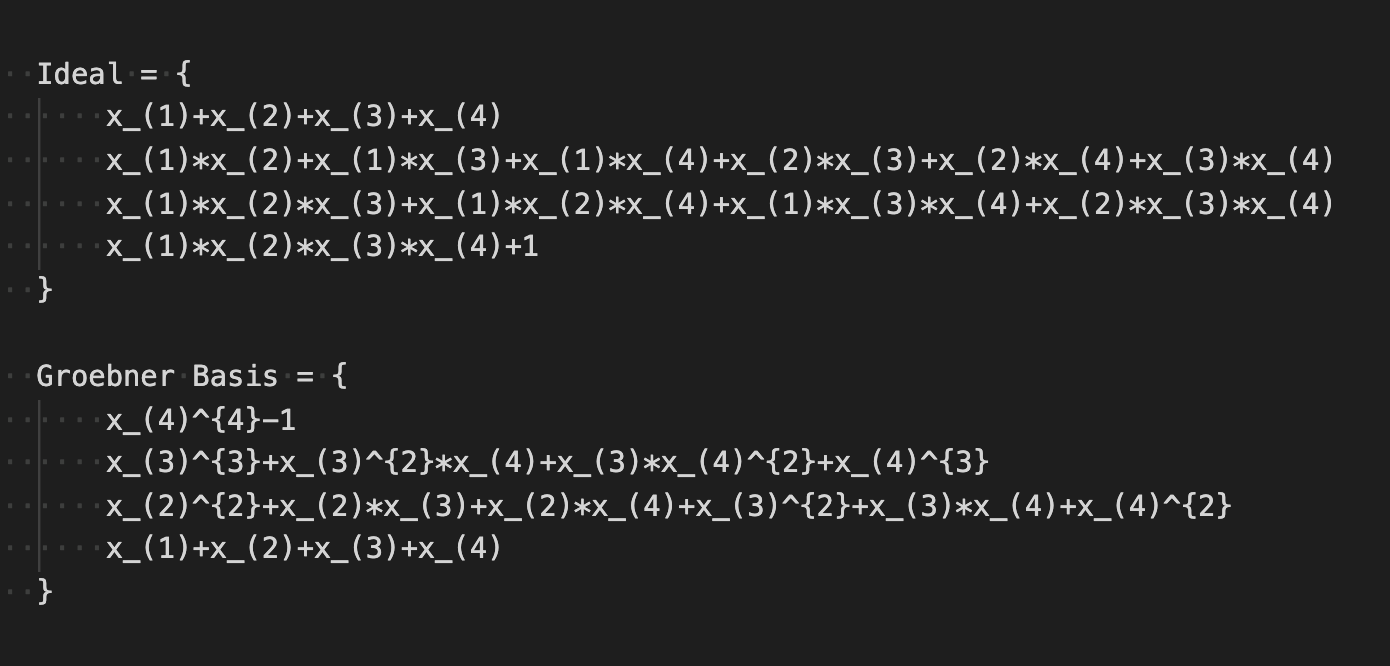
\includegraphics[scale=0.45]{Example.png}
%         \centering
%     \end{figure}
% \end{frame}

% \begin{frame}{Чего удалось достичь}
%     Benchmark from Root 6 to Root 8 ($\mathbb{R}[x_1, \ldots, x_n]$, порядок: Lex):
%     \begin{figure}[t]
%         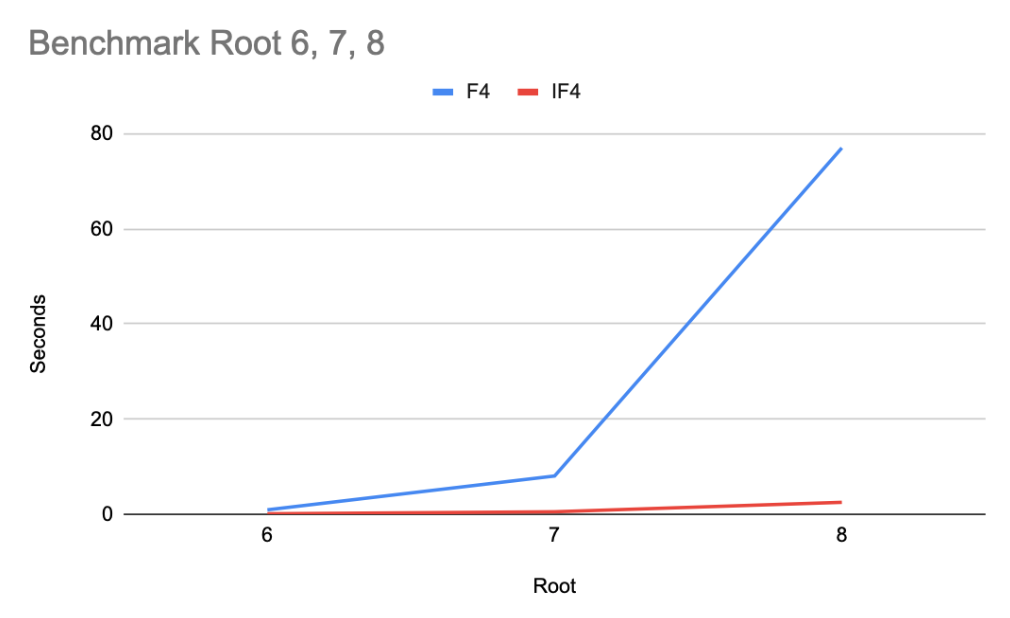
\includegraphics[scale=0.6]{Benchmark6.png}
%         \centering
%     \end{figure}
% \end{frame}

% \begin{frame}{Чего удалось достичь}
%     Benchmark from Root 9 to Root 13 ($\mathbb{R}[x_1, \ldots, x_n]$, порядок: Lex):
%     \begin{figure}[t]
%         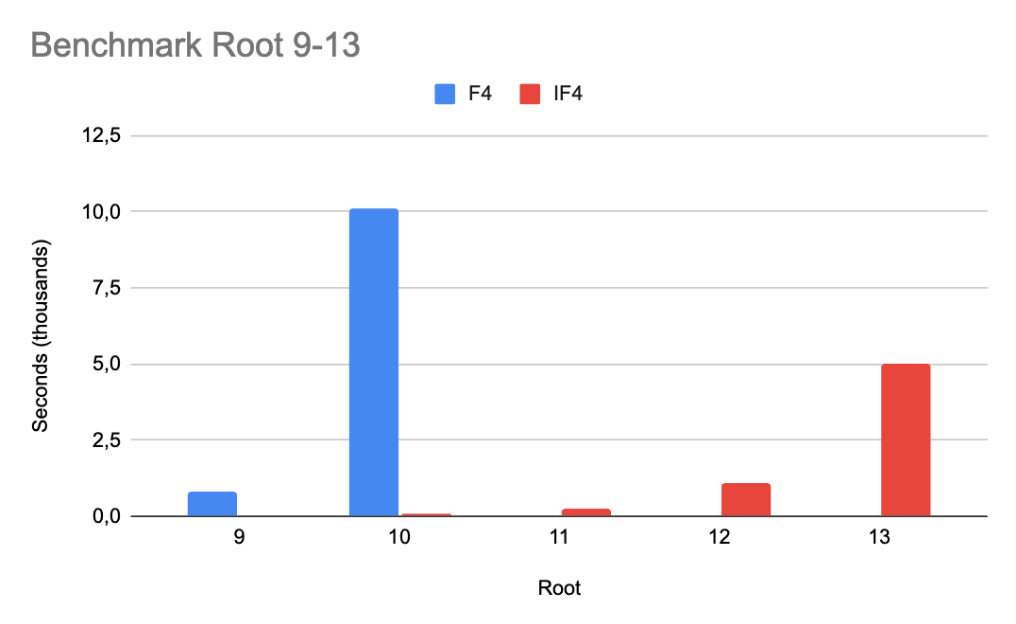
\includegraphics[scale=0.6]{Benchmark13.png}
%         \centering
%     \end{figure}
% \end{frame}

% \begin{frame}{Чего удалось достичь}
%     Benchmark Buchberger Criterion \& IF4 ($\mathbb{R}[x_1, \ldots, x_n]$, порядок: Lex):
%     \begin{figure}[t]
%         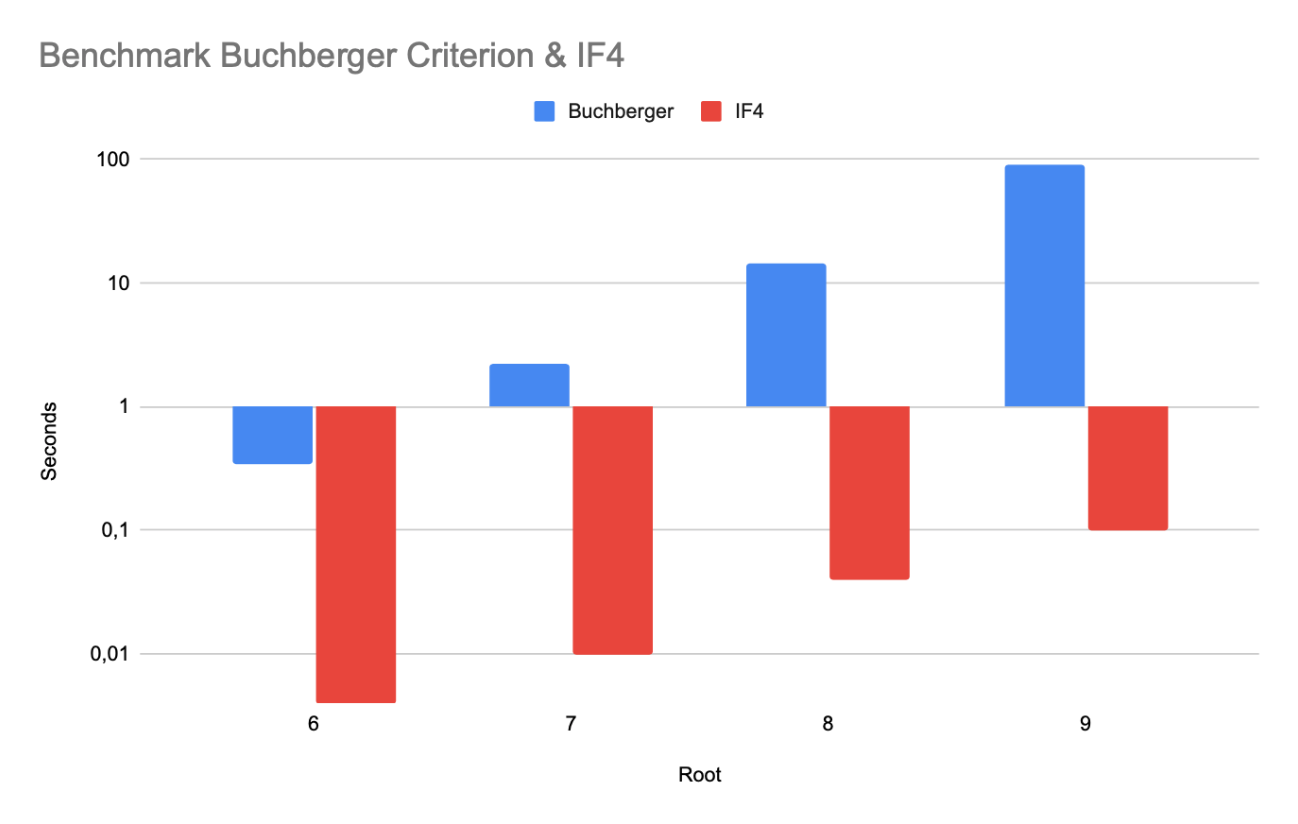
\includegraphics[scale=0.4]{criterion.png}
%         \centering
%     \end{figure}
% \end{frame}

\end{document}
